% The paper followed by its supplementary material, in one file. Build as main.tex and supplement.tex, then
% tectonic -X compile full.tex.
\documentclass[11pt]{article}
% Shared by main.tex (the paper), supplement.tex (the supplement on its own) and full.tex (both in one file).
\usepackage[margin=1in]{geometry}
\usepackage{fontspec}
\usepackage{microtype}
\usepackage{amsmath,amssymb}
\usepackage{booktabs}
\usepackage{array}
\usepackage{calc}
\usepackage{tabularx}
\usepackage{graphicx}
\usepackage{xcolor}
\usepackage{caption}
\usepackage{enumitem}
\usepackage{seqsplit}
\usepackage{tikz}
\usetikzlibrary{positioning,arrows.meta,calc,fit,backgrounds}
\usepackage[colorlinks=true,linkcolor=blue!50!black,citecolor=blue!50!black,urlcolor=blue!50!black]{hyperref}

\captionsetup{font=small,labelfont=bf}
\setlist{itemsep=1pt,topsep=3pt}
\providecommand{\tightlist}{\setlength{\itemsep}{1pt}\setlength{\parskip}{0pt}}
% pandoc column widths, (\linewidth - 2n\tabcolsep) * \real{share}, need calc
\setlength{\emergencystretch}{2em}

\newcommand{\papertitle}{Contain, Conform, Compare: A Red-Teamed Kit for Evaluating Small Coding Agents on One GPU}
\newcommand{\papersubtitle}{Attacked per-job containers, token-level prompt checks, and a pre-registered test of four prompt divergences}

\newcommand{\paperauthor}{Nguyen Minh Thang\\
\small VNU University of Science, 334 Nguyen Trai, Thanh Xuan, Hanoi, Vietnam}
\newcommand{\paperdate}{November 2026}
\newcommand{\repourl}{https://github.com/MinhThanghus/drydock-eval}

% The supplement numbers its sections, tables and figures S1, S2, ... in every build.
\newcommand{\supplementnumbering}{%
  \setcounter{section}{0}\setcounter{table}{0}\setcounter{figure}{0}%
  \renewcommand{\thesection}{S\arabic{section}}\renewcommand{\thetable}{S\arabic{table}}\renewcommand{\thefigure}{S\arabic{figure}}%
  \renewcommand{\theHsection}{S\arabic{section}}\renewcommand{\theHtable}{S\arabic{table}}\renewcommand{\theHfigure}{S\arabic{figure}}}

\newcommand{\papersec}[1]{Section~\ref{sec:#1}}
\newcommand{\papertab}[1]{Table~\ref{tab:#1}}
\newcommand{\paperfig}[1]{Figure~\ref{fig:parity}}
\newcommand{\papercite}[2]{\cite{#1}}

\title{\papertitle\\[6pt]
\large \papersubtitle}
\author{\paperauthor}
\date{\paperdate}

\begin{document}
\maketitle

\begin{abstract}
A hosted score in the Gemma 4 Developer Agent competition \cite{r1} is one noisy number, so development needs a local evaluator that is fast, safe for agent-written code, and matching the hosted scorer's prompts. \texttt{drydock-eval} evaluates a small coding agent (Gemma 4 E4B \cite{r2}) at about 250 runs per hour on one RTX 5090. \emph{Contain} runs each job in a fresh container without network and passed 200 scripted escape tests; \emph{conform} provides eight checks that compare a local stack's requests with the scorer's configuration, down to rendered tokens; \emph{compare} provides paired statistics that respect repository clusters. AI agents built and attacked the kit; a human owner approved machine use and release. Across seven runner versions no attack escaped the container's namespaces or privileges, yet nine demonstrated high-severity vectors came through what the host shared with it, in designs passing their own escape tests; the last independent verifier found no high or medium issue. Rendered prompts matched the Kaggle template on 396 of 396 requests by token count and 50 of 50 by token id. A pre-registered five-arm experiment (231 tasks, 4,620 jobs) measured four prompt divergences: no E4B solve-rate change was detected (largest estimate \ensuremath{-}2.1 points, 95\% interval \ensuremath{-}4.4 to +0.4).
\end{abstract}

\section{Introduction}\label{sec:1}

The competition scores an agent bundle on hidden GitHub-issue tasks, with Gemma 4 served by vLLM \cite{r11}. Third-party analyses put the noise of one hosted score near 1.5 of 58 tasks \cite{r3,r4}. Local evaluation must therefore carry development; on a Kaggle kernel with four L4 GPUs our stack finished 35.2 agent runs per hour, serially.

\textbf{Safety.} An agent run executes model-written shell commands and installs model-edited packages; our first local setup ran them with no sandbox.

\textbf{Fidelity.} We call a \emph{rendering trap} a configuration detail that silently changes the token sequence the model receives while runs still finish and score. The \emph{scorer path} is the scorer's configuration reproduced locally. In our first setup the served model name contained ``gemma4'', so the agent framework (google-adk 1.36.1) sent tool results with role \texttt{tool\_responses} instead of \texttt{tool} \cite{r5}. Prompts rebuilt from its traces matched the server's token counts on 106 of 114 calls only when rendered with \texttt{tool\_responses} (0 of 114 with \texttt{tool}). Solve counts hid it: that setup solved 3 and 5 of 24 tasks against 4 and 4 on Kaggle (Fisher p 0.74 and 0.75).

These traps are public: the role rule \cite{r5}, thought handling in history \cite{r6,r7,r8}, a newline after thinking text \cite{r9}, and the scorer's compaction settings \cite{r10}. We discovered none of them; we contribute checks that detect them (\S\ref{sec:4}) and a measurement of three of them plus a template swap (\S\ref{sec:6}).

\section{Scope, threat model and rules}\label{sec:2}

% Figure: where the three modules sit. Every label restates Sections 3-5; no number here is new.
\begin{figure}[!tb]
\centering
\footnotesize
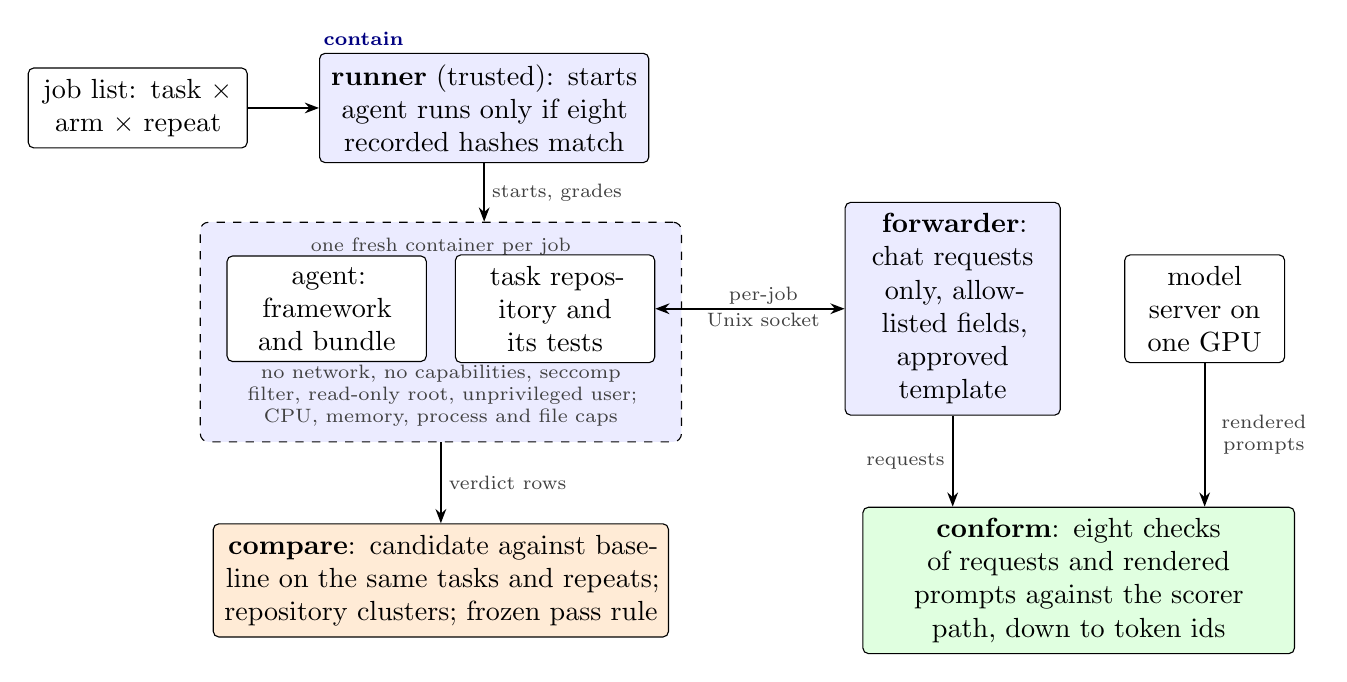
\begin{tikzpicture}[
  box/.style={draw, rounded corners=2pt, align=center, inner sep=4pt, text width=#1, minimum height=0.95cm},
  con/.style={box=#1, fill=blue!8},
  cfm/.style={box=#1, fill=green!12},
  cmp/.style={box=#1, fill=orange!16},
  plain/.style={box=#1, fill=white},
  arr/.style={-{Stealth[length=1.8mm]}, thick},
  darr/.style={{Stealth[length=1.8mm]}-{Stealth[length=1.8mm]}, thick},
  lab/.style={font=\scriptsize, align=center, inner sep=1.5pt, text=black!75}]
% row 1: what starts a job
\node[plain=2.5cm] (jobs)   at (1.2,0)    {job list: task $\times$ arm $\times$ repeat};
\node[con=3.9cm]   (runner) at (5.6,0)    {\textbf{runner} (trusted): starts agent runs only if eight recorded hashes match};
% row 2: the job
\node[lab, anchor=south] (ctrlab) at (5.05,-1.93) {one fresh container per job};
\node[plain=2.25cm] (agent) at (3.6,-2.55) {agent: framework and bundle};
\node[plain=2.25cm] (repo)  at (6.5,-2.55) {task repository and its tests};
\node[lab, anchor=north, text width=5.5cm] (restr) at (5.05,-3.2)
  {no network, no capabilities, seccomp filter, read-only root, unprivileged user; CPU, memory, process and file caps};
\begin{scope}[on background layer]
\node[draw, dashed, rounded corners=3pt, fill=blue!8, inner xsep=7pt, inner ysep=4pt, fit=(ctrlab)(agent)(repo)(restr)] (ctr) {};
\end{scope}
\node[con=2.45cm] (fwd) at (11.55,-2.55) {\textbf{forwarder}: chat requests only, allow-listed fields, approved template};
\node[plain=1.75cm] (srv) at (14.75,-2.55) {model server on one GPU};
% row 3: what reads the outputs
\node[cmp=5.5cm] (cmpn) at (5.05,-6.0)  {\textbf{compare}: candidate against baseline on the same tasks and repeats; repository clusters; frozen pass rule};
\node[cfm=5.2cm] (cfmn) at (13.15,-6.0) {\textbf{conform}: eight checks of requests and rendered prompts against the scorer path, down to token ids};
% arrows
\draw[arr] (jobs) -- (runner);
\draw[arr] (runner.south) -- node[lab, right, xshift=1pt] {starts, grades} (runner.south |- ctr.north);
\draw[darr] (repo.east) -- (fwd.west);
\path (ctr.east |- repo.east) -- node[lab, above] {per-job} node[lab, below] {Unix socket} (fwd.west);
\draw[arr] (ctr.south) -- node[lab, right, xshift=1pt] {verdict rows} (ctr.south |- cmpn.north);
\draw[arr] (fwd.south) -- node[lab, left, xshift=-1pt] {requests} (fwd.south |- cfmn.north);
\draw[arr] (srv.south) -- node[lab, right, xshift=1pt, text width=1.3cm] {rendered prompts} (srv.south |- cfmn.north);
% module tag
\node[lab, anchor=south west, text=blue!50!black] at ([yshift=1pt]runner.north west) {\textbf{contain}};
\end{tikzpicture}
\caption{The kit: where each module sits.}
\label{fig:overview}
\end{figure}


\textbf{Stack.} Gemma 4 E4B, 4-bit quantization-aware checkpoint (Kaggle model version 2); vLLM 0.19.1; google-adk 1.36.1; the competition's harness packages. Tasks come from Berth \cite{r12}: 579 of its 653 tasks load in the harness and pass our validation (the reference patch passes, an empty patch fails). Experiments ran on a shared single-GPU workstation (RTX 5090, 32 GB).

\textbf{Threat model.} The adversary is the code the agent writes. It may try to read host files or other jobs, reach the network, exhaust host resources, forge its verdict, or outlive its job. Kernel exploits are out of scope.

\textbf{Who did the work.} AI agents wrote the kit's code, attacks and analyses (builders). Separate AI agents (verifiers) re-implemented or re-ran the work adversarially. A lead AI session froze the protocols; a human owner approved isolation, machine time and release. ``Verified'' below means this process, not human review.

\section{Contain: a runner and the attacks it failed}\label{sec:3}

In the final design each job gets one fresh container: no network, no capabilities, a seccomp filter, a read-only root, an unprivileged user, 2 CPUs, 10 GiB of memory, 4,096 processes, and temporary filesystems capped in bytes and inodes. The only request channel is a per-job Unix socket to a forwarder, which passes only chat-completion requests with allow-listed fields, text-only content and an approved template hash, under rate and size caps. Agent runs start only if eight recorded hashes (image, code, flags, model files) still match.

A \emph{canary} is a scripted attack with a machine-checked outcome.

\begin{table}[!tb]
\centering
\caption{Runner versions.}\label{tab:1}
\footnotesize
\begin{tabular}{@{}
  >{\raggedright\arraybackslash}p{(\linewidth - 4\tabcolsep) * \real{0.2000}}
  >{\raggedright\arraybackslash}p{(\linewidth - 4\tabcolsep) * \real{0.1900}}
  >{\raggedright\arraybackslash}p{(\linewidth - 4\tabcolsep) * \real{0.6100}}@{}}
\toprule
\begin{minipage}[b]{\linewidth}\raggedright
Runner version
\end{minipage} & \begin{minipage}[b]{\linewidth}\raggedright
Canaries passed
\end{minipage} & \begin{minipage}[b]{\linewidth}\raggedright
Security findings of independent verifiers
\end{minipage} \\
\midrule
1. Container per command & 52/52 & 4 high: host-side install ran the agent's \texttt{setup.py} (builder-found); symlink leaked a host file; 10 GiB of host disk reserved in 0.005 s; host copied a sparse file in full \\
2. Hardened, per command & 60/60 (57/60 before canary fixes) & 4 high, 1 untested: host overwrote a file through a planted link; cleanup followed links; 6 GiB reserved in 0.012 s; 200,000 files in 2.4 s \\
3. Container per job & 98/98 & 1 high: the model server could fetch URLs named in requests; 2 medium \\
4--6. Request filter added, tightened & 134/134, 159/159, 191/191 & medium at most \\
7. Final & 200/200 & no high or medium \\
\bottomrule
\end{tabular}
\end{table}

\begin{figure}[!tb]
\centering
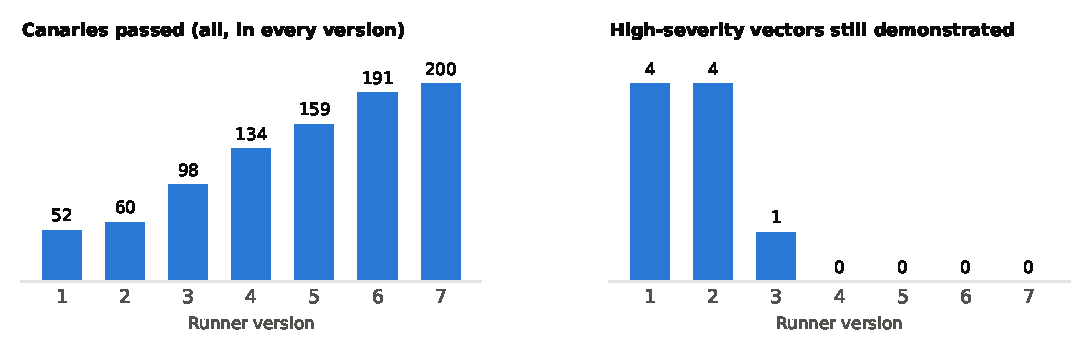
\includegraphics[width=\linewidth]{fig/runner_versions.pdf}
\caption{Canaries passed and high-severity vectors found, per runner version.}
\label{fig:versions}
\end{figure}


\textbf{Passing canaries proved little.} No attack escaped the container's namespaces or privileges in any round. Nine demonstrated high-severity vectors came through what the host shared with it: host-side steps that touched agent-written files, resource limits (a known class \cite{r13}) and the model server.

\textbf{Final version.} Controls on 481 tasks (reference patch 481/481, empty patch 0/481) showed no verdict, exit-code or test-summary difference from the previous version. After the runner was killed, the container was gone within 149 s with no further model request. The final runner completed a 24-job list at 251--254 runs per hour with 8 workers.

\textbf{What remains.} Containers share the host kernel; user namespaces are not remapped; the request parser runs in the trusted runner; a job can slow others through the shared model server within its caps. Our claim is conditional: against the stated adversary and with the eight hashes matching, no tested attack succeeded.

\section{Conform: eight checks against the scorer path}\label{sec:4}

\texttt{conform} reads the requests a local stack sent and, where logged, the prompts the server rendered. Reference values come from the public starter notebook \cite{r10}, our Kaggle-kernel traces, and the Kaggle model's chat template.

\begin{table}[!tb]
\centering
\caption{The eight checks.}\label{tab:2}
\footnotesize
\begin{tabular}{@{}
  >{\raggedright\arraybackslash}p{(\linewidth - 4\tabcolsep) * \real{0.1300}}
  >{\raggedright\arraybackslash}p{(\linewidth - 4\tabcolsep) * \real{0.5200}}
  >{\raggedright\arraybackslash}p{(\linewidth - 4\tabcolsep) * \real{0.3500}}@{}}
\toprule
\begin{minipage}[b]{\linewidth}\raggedright
Check
\end{minipage} & \begin{minipage}[b]{\linewidth}\raggedright
Compares
\end{minipage} & \begin{minipage}[b]{\linewidth}\raggedright
Mutation runs caught
\end{minipage} \\
\midrule
role & role of tool results & 53/53 \\
sampling & temperature, top-p, token and thinking budgets & 52/52 \\
tools & declared tool schemas & 20/20 \\
shape & message skeleton, system text, field encoding & 72/72 \\
template & rendered prompt against the Kaggle template & 13/21 by token count, 24/24 by token id \\
thoughts & history thoughts, under the key the server reads & 52/52 \\
newline & newline before the token closing a thought & 12/12 \\
compaction & when history is summarized (14,336 tokens \cite{r10}) & 19/19 \\
\bottomrule
\end{tabular}
\end{table}

\textbf{Role.} From each google-adk release's source (only 1.36.1 was executed): 1.34.0--1.39.1 and 2.0--2.4 send \texttt{tool\_responses} when the model string contains ``gemma4''; 2.5--2.11 when it matches \texttt{gemma-?4}; 2.12--2.14 exempt three OpenAI-compatible providers \cite{r5}. The harness packages require \texttt{\textgreater{}=1.34.0,\textless{}2.0}.

\textbf{Thoughts.} vLLM 0.19.1 reads an earlier assistant thought only from the field \texttt{reasoning}. google-adk 1.36.1 writes \texttt{reasoning\_content}, which that server drops silently \cite{r8}; the competition harness writes both. Removing \texttt{reasoning} in a probe lost 55 of 55 thoughts from the rendered prompt.

\textbf{Template.} The check re-renders each request outside vLLM with the Kaggle template and compares token counts with the server's, or token ids when the server logs them, because identical strings can tokenize differently \cite{r16}.

\textbf{Evidence.} In version 2's 24-task parity run, all 2,566 tool results had role \texttt{tool}, and re-rendering reproduced the server's token count on 396 of 396 requests (with \texttt{tool\_responses}: 0 of 358 multi-turn requests). With the final runner, the checker reproduced the token ids of 243 of 243 returned calls, and a renderer written separately by the verifier matched 50 of 50 scorer-path requests. Prompts rebuilt from early calls of our Kaggle-kernel traces match the recorded counts on 181 of 189 calls with role \texttt{tool} and thoughts kept, 1 of 189 with \texttt{tool\_responses} and 0 of 189 with thoughts dropped: our only Kaggle-side evidence, and count-level.

\textbf{Mutation suite.} 103 mutations (85 drifts, 18 benign controls) in four scripted scenarios against a mock server give 412 runs. The intended check caught 317 of 325 applicable drift runs; the 8 misses are same-length template changes seen through counts only. No check failed in 72 control runs (24 warned).

\section{Compare: a decision rule that respects repositories}\label{sec:5}

Tasks from one repository succeed and fail together. Clustered inference for model evaluations is prior art \cite{r19}; \texttt{compare} packages a small-cluster version with a frozen pass rule and its simulated behaviour.

Candidate and baseline run on the same tasks and repeats. A candidate passes only if (1) the mean gain is at least 2/58 (3.45 points, two leaderboard tasks); (2) one-sided p \ensuremath{\le} 0.025 under a null-imposed wild cluster bootstrap-t over repositories, with Rademacher weights and 9,999 draws \cite{r20,r21}; (3) at least three repositories gain and every leave-one-repository-out estimate is positive; (4) agent time stays within 1.2 times baseline and infrastructure errors do not rise; and (5) no repository loses two task-equivalents or more. Two panels were frozen before any outcome: a small one (72 tasks, 18 repositories) and a large one (200 tasks, 20 repositories).

\begin{table}[!tb]
\centering
\caption{Simulated pass rates (3,000 simulations per cell; 400 for the dropping row).}\label{tab:3}
\footnotesize
\begin{tabular}{@{}
  >{\raggedright\arraybackslash}p{(\linewidth - 4\tabcolsep) * \real{0.5800}}
  >{\raggedright\arraybackslash}p{(\linewidth - 4\tabcolsep) * \real{0.2100}}
  >{\raggedright\arraybackslash}p{(\linewidth - 4\tabcolsep) * \real{0.2100}}@{}}
\toprule
\begin{minipage}[b]{\linewidth}\raggedright
Simulated scenario
\end{minipage} & \begin{minipage}[b]{\linewidth}\raggedright
Small panel
\end{minipage} & \begin{minipage}[b]{\linewidth}\raggedright
Large panel
\end{minipage} \\
\midrule
No effect, exchangeable tasks & 0.23--1.90\% & 0.00--0.50\% \\
No mean effect, candidate breaks 20\% of repositories & 7.50\% & 8.43\% \\
No effect, worst tasks dropped after seeing outcomes & 31.75\% & 40.75\% \\
Even gain of 3/58 (power) & \ensuremath{\approx}60\% & \ensuremath{\approx}90\% \\
Gain confined to four repositories (power) & 15.9\% & 24.9\% \\
\bottomrule
\end{tabular}
\end{table}

The 2.5\% level holds for exchangeable effects, not for skewed ones, and not if tasks are dropped after unblinding. Independent re-implementations matched the rule code on 280 of 280 clean datasets (first version) and, with rule readings aligned, 193 of 194 (amended). Applied three times, to screen leaders from one separate 48-task set (25, 22, 25 of 96 runs solved; baselines 19, 21, 20); none passed. Gains: \ensuremath{-}0.35 points on the small panel (p = 0.60); on the 128 large-panel tasks outside it, \ensuremath{-}0.39 (p = 0.60), then +4.10 (p = 0.04 \textgreater{} 0.025, uncorrected). Condition (5): first application only.

\section{Case study: four prompt divergences on E4B}\label{sec:6}

Five arms share one model server, one withheld agent bundle, google-adk 1.36.1 and all sampling settings.

\begin{table}[!tb]
\centering
\caption{Arms; changes in percentage points.}\label{tab:4}
\footnotesize
\begin{tabular}{@{}
  >{\raggedright\arraybackslash}p{(\linewidth - 6\tabcolsep) * \real{0.0500}}
  >{\raggedright\arraybackslash}p{(\linewidth - 6\tabcolsep) * \real{0.4000}}
  >{\raggedright\arraybackslash}p{(\linewidth - 6\tabcolsep) * \real{0.1900}}
  >{\raggedright\arraybackslash}p{(\linewidth - 6\tabcolsep) * \real{0.3600}}@{}}
\toprule
\begin{minipage}[b]{\linewidth}\raggedright
Arm
\end{minipage} & \begin{minipage}[b]{\linewidth}\raggedright
Difference from the scorer path
\end{minipage} & \begin{minipage}[b]{\linewidth}\raggedright
Requests changed by the divergence
\end{minipage} & \begin{minipage}[b]{\linewidth}\raggedright
Change against F {[}95\% interval{]}; Holm p
\end{minipage} \\
\midrule
F & none: role \texttt{tool}, Kaggle template, compaction at 14,336 tokens, thoughts under both keys & --- & solve rate 23.8\% \\
R & model name contains ``gemma4'': tool results get role \texttt{tool\_responses} & 89\% & \ensuremath{-}0.3 {[}\ensuremath{-}2.8, +2.2{]}; p = 1 \\
C & compaction unset: prompts grow until rejected above 24,576 tokens (the run ends; edits are still graded) & 21\% & +0.2 {[}\ensuremath{-}2.0, +2.5{]}; p = 1 \\
H & history thoughts removed from every request, as when a client omits the key the server reads & 90\% & \ensuremath{-}2.1 {[}\ensuremath{-}4.4, +0.4{]}; p = 0.44 \\
T & the Hugging Face E4B template: a thought opener is forced after each tool result & 85\% & +0.8 {[}\ensuremath{-}1.4, +2.9{]}; p = 1 \\
\bottomrule
\end{tabular}
\end{table}

No newline arm was run: both templates render it identically on this server.

\textbf{Panel.} Removing tasks used by other panels, reserved repositories, slow tasks and duplicates from the 579 leaves 231 tasks in 15 repositories. They run 4 repeats in 5 arms (4,620 jobs); for each task and repeat the arms run back to back in counterbalanced order.

\textbf{Analysis, frozen before any outcome} (protocol sha256 \texttt{\seqsplit{070c9655d96372d054f430727259de7b25af2ca93c3ec4c9295dfdc37aeb8cf4}}). The estimand $d_X$ is the mean over tasks of arm X's solve rate minus arm F's. The primary test is an exact two-sided task-level sign-flip test, Holm-corrected over the four arms at 0.05; only then do we say that X raises or lowers E4B's solve rate \emph{on these tasks}. Intervals (unadjusted) invert that test. A repository-cluster bootstrap interval is secondary (lower simulated power). A frozen checker re-renders every returned request from the job's dump, matches the server's token count and confirms the job's arm; a failing job is re-run. Outcomes stayed blind until a pre-registered cut-off (2026-11-11 06:00 UTC) and were unblinded once.

\textbf{Power, simulated before data.} The family-wise false-claim rate is 1.2--4.2\%. At 231 tasks an even 5-point drop in one arm is detected with probability 82--100\% across the simulated settings; the drop or gain detected with 80\% power ranges from below 3 to about 5.2 points.

\textbf{Deviations recorded blind.} Independent validation of the final runner finished only after launch. From about an hour in, a second workload held about 9.6 GiB of GPU memory, so timings are under mixed load. The block stopped three times: after 967 jobs at the runner's open-file limit (cause unknown), after 378 more by an external termination signal on the shared machine, and after 3,074 more when the kernel's out-of-memory killer ended the model server (cause undiagnosed). Each resume ran only never-started jobs; the 24 interrupted jobs were re-run once.

\textbf{Results.} All jobs finished before the cut-off. Every arm has a valid row in 924 of 924 slots, and the checker passed all 4,620 analysed jobs. No pre-emption was recorded; 6.0\% of runs took over 240 s, above the pre-registered 5\% threshold. No difference from F was detected for any arm (Table~\ref{tab:4}, Figure~\ref{fig:parity}B; smallest Holm-adjusted p 0.44); the secondary repository-cluster intervals all include zero. The largest estimate is H's \ensuremath{-}2.1 points (unadjusted p 0.11; \ensuremath{-}1.3 with time-limit rows as missing). In exploratory measures, H runs averaged 137 s against 78 s and ended unsolved at the bundle's five-minute limit in 11.5\% of runs against 1.8\%; in C, 12.3\% of runs ended unsolved on a rejected over-long prompt. These are null results, not evidence of no effect: the simultaneous 98.75\% intervals allow a drop of 5.1 points (H) and a gain of 3.5 (T).

\begin{figure}[!tb]
\centering
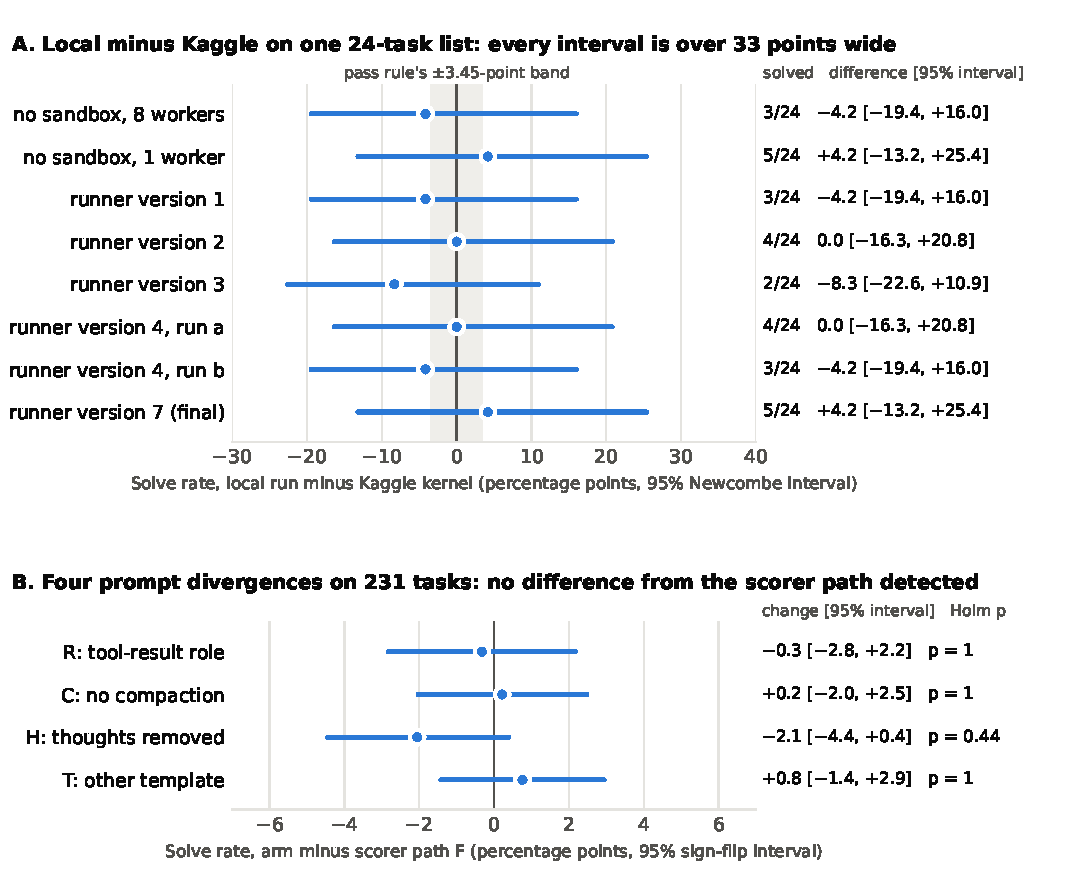
\includegraphics[width=\linewidth]{fig/parity_effects.pdf}
\caption{(A) Solve-rate difference, local minus Kaggle (pooled 8/48), for eight local runs of one 24-task list (95\% Newcombe intervals, runs treated as independent); shaded: the pass rule's \ensuremath{\pm}3.45 points. (B) Change in solve rate against F on 231 tasks: estimates, 95\% intervals and Holm-adjusted p.}\label{fig:parity}
\end{figure}

\section{Related work}\label{sec:7}

SandboxEval \cite{r14} and SandboxEscapeBench \cite{r15} test sandboxes and models' ability to escape them.

Several paper-track resources overlap this one (described from their public text only): LAB \cite{r22}, a Docker sandbox with 11 tests and a bundle gate with 16 detectors validated by fault injection; Szeto et al.'s cloud rig with 141 run folders \cite{r23}; gemma4-swe-kit \cite{r17}, a proxy reproducing the scorer's template, call parsing and compaction on other servers; a dataset card reporting count parity on 107 captured vLLM requests \cite{r18}; Silent Zeros \cite{r24}, a bundle checker tested on 22 broken bundles; and ThoughtKeep \cite{r25}, 1,470 Gemma 4 31B attempts on thought retention. We did not find in those texts, and offer here: a runner attacked by independent verifiers with its canary misses published, token-id comparison backed by a mutation suite, and a trap measurement on E4B with a per-job prompt check.

\section{Limitations}\label{sec:8}

\begin{itemize}
\tightlist
\item
  \textbf{Solve-level parity is not refuted, not established.} The evidence (Figure~\ref{fig:parity}A) is one 24-task list, one repeat per run; ten runs solved only six distinct tasks.
\item
  \textbf{Kaggle-side facts are partly inferred}: the hosted google-adk release, tool-schema equality, and the identity of the hosted template and weights with the public Kaggle model.
\item
  \textbf{Environment differences remain.} One RTX 5090 instead of four L4s; 2 CPUs and 10 GiB per job; a bare \texttt{pytest} command, used in 30 of 216 commands in our Kaggle traces, is absent locally.
\item
  \textbf{The case study} covers one model, one bundle, one google-adk release and one configuration per divergence. Arm T swaps a whole template; in arm H thoughts still reach compaction summaries.
\end{itemize}

\section{Availability}\label{sec:9}

\texttt{drydock-eval} 0.4.0 (Apache-2.0) has three modules: \texttt{conform} (checks, mock server, mutation suite), \texttt{contain} (a reference runner tree, its escape tests, a gate helper) and \texttt{compare} (pass rule, sign-flip tests, simulations). Its 435 CPU tests pass. The released runner has not been run in a container as released: the 200 of 200 result is for the deployed tree, of which the release is an identifier-substituted copy with two canaries rewritten. Code: \url{https://github.com/MinhThanghus/drydock-eval} (tag \texttt{v0.4.0}; branch \texttt{paper}: supplement, \S\ref{sec:6} outcome rows). The package also carries copies of the \S\ref{sec:6} protocol, analysis code and job-list generator, redacted where needed, each with its original's sha256; the agent bundle and request dumps are planned for 2026-12-03.

\begin{thebibliography}{25}
\small
\bibitem{r1} Google DeepMind. \href{https://www.kaggle.com/competitions/gemma-4-developer-agent}{Gemma 4 Developer Agent Competition}. Kaggle, 2026.
\bibitem{r2} Gemma Team. Gemma 4 Technical Report. arXiv:2607.02770, 2026.
\bibitem{r3} dariushafshar. \href{https://www.kaggle.com/datasets/dariushafshar/gemma-4-agent-public-config-draws}{Gemma 4 Agent: Public Config Draws}. Kaggle, 2026.
\bibitem{r4} Mobassir. \href{https://www.kaggle.com/datasets/mobassir/swe-agent-eval-validity-gemma4}{Too Small to See}. Kaggle, 2026.
\bibitem{r5} rladeira. \href{https://github.com/google/adk-python/issues/7977}{google/adk-python issue \#7977}. 2026.
\bibitem{r6} Google. \href{https://ai.google.dev/gemma/docs/core/prompt-formatting-gemma4}{Gemma 4 Prompt Formatting}. 2026.
\bibitem{r7} dimondev. \href{https://huggingface.co/google/gemma-4-E2B-it/discussions/44}{Hugging Face gemma-4-E2B-it pull request \#44}. 2026.
\bibitem{r8} delta9000. \href{https://github.com/vllm-project/vllm/issues/38488}{vLLM issue \#38488}. 2026.
\bibitem{r9} G. Gerganov. \href{https://huggingface.co/google/gemma-4-31B-it/discussions/135}{Hugging Face gemma-4-31B-it discussion \#135}. 2026.
\bibitem{r10} ryanholbrook. \href{https://www.kaggle.com/code/ryanholbrook/getting-started-gemma-4-developer-agent}{Getting Started - Gemma 4 Developer Agent}. Kaggle, 2026.
\bibitem{r11} W. Kwon et al.~Efficient Memory Management for Large Language Model Serving with PagedAttention. SOSP 2023.
\bibitem{r12} J. Patel. \href{https://www.kaggle.com/datasets/jayp2005/berth-swe-tasks}{Berth}. Kaggle, 2026.
\bibitem{r13} X. Gao et al.~Houdini's Escape. CCS 2019.
\bibitem{r14} R. Rabin et al.~SandboxEval. arXiv:2504.00018, 2025.
\bibitem{r15} R. Marchand et al.~Quantifying Frontier LLM Capabilities for Container Sandbox Escape. ICML 2026.
\bibitem{r16} Agent Lightning Team. \href{https://vllm.ai/blog/2025-10-22-agent-lightning}{No More Retokenization Drift}. 2025.
\bibitem{r17} damsolanke. \href{https://github.com/damsolanke/gemma4-swe-kit}{gemma4-swe-kit}. GitHub, 2026.
\bibitem{r18} tyfeng1997. \href{https://huggingface.co/datasets/tyfeng1997/gemma4-e4b-swe-sft-32k-competition-template}{gemma4-e4b-swe-sft-32k-competition-template}. Hugging Face, 2026.
\bibitem{r19} E. Miller. Adding Error Bars to Evals. arXiv:2411.00640, 2024.
\bibitem{r20} A. Cameron, J. Gelbach, D. Miller. Bootstrap-Based Improvements for Inference with Clustered Errors. REStat, 2008.
\bibitem{r21} J. MacKinnon, M. Webb. Wild Bootstrap Inference for Wildly Different Cluster Sizes. J. Applied Econometrics, 2017.
\bibitem{r22} marcofpereira. \href{https://www.kaggle.com/datasets/marcofpereira/gemma4-lab-v1}{Gemma 4 Developer Agent LAB}. Kaggle, 2026.
\bibitem{r23} J. Szeto, D. Guo, H. Szeto. \href{https://www.kaggle.com/datasets/jaydenszeto123/gemma-4-developer-agent-scorer-faithful-rig}{Scorer-Faithful Local Evaluation for Small Coding Agents}. Kaggle, 2026.
\bibitem{r24} houchiunyo. \href{https://www.kaggle.com/datasets/houchiunyo/gemma4-agent-silent-zeros}{Gemma 4 agent resource: runs \& checker}. Kaggle, 2026.
\bibitem{r25} hemantkumarbk. \href{https://www.kaggle.com/datasets/hemantkumarbk/thoughtkeep-reproduction-inputs}{Coding-Agent Thought Retention: Reproduction Data}. Kaggle, 2026.
\end{thebibliography}


\clearpage
\begin{center}
{\Large\bfseries Supplementary material}
\end{center}
\supplementnumbering
% Supplementary material: body. Used by supplement.tex (on its own) and full.tex (after the paper).
% Every table is written by supp/build_supp.py or supp/reproduce.py (gen/s_*.tex). Every number in the prose is a macro
% written by those scripts (gen/supp_macros.tex, gen/repro_macros.tex, gen/gate_macros.tex) or restates a sentence of
% the paper; supp/gates_text.tex names the few numbers that come from recorded screen analyses.
\newcommand{\SLoadRows}{4{,}620}
\newcommand{\SLoadFlag}{5}
\newcommand{\SInfraNoRow}{8}
\newcommand{\SReRuns}{24}
\newcommand{\STasksNever}{135}
\newcommand{\STasksAlways}{13}
\newcommand{\STasksMixed}{83}
\newcommand{\SHTasksDown}{34}
\newcommand{\SHTasksUp}{20}
\newcommand{\SRunsPerArm}{924}
\newcommand{\SCRejectedShare}{12.3}
\newcommand{\SHUnsolvedAtLimitShare}{11.5}
\newcommand{\SFUnsolvedAtLimitShare}{1.8}
\newcommand{\SFCompactedShare}{48}
\newcommand{\SFailedCalls}{299}
\newcommand{\SHLooLo}{3.01}
\newcommand{\SHLooHi}{1.44}
\newcommand{\SFRate}{23.8}
\newcommand{\SMinRate}{21.8}
\newcommand{\SMaxRate}{24.6}
\newcommand{\SFirstStart}{2026-11-10 06:39}
\newcommand{\SLastEnd}{2026-11-11 03:56}
\newcommand{\SExposureMin}{85}
\newcommand{\SExposureMax}{90}
\newcommand{\SRows}{4{,}636}
\newcommand{\SAgentRows}{4{,}620}
\newcommand{\SInfraRowsWritten}{16}
\newcommand{\SInfraRowsAll}{24}
\newcommand{\SJobsStarted}{4{,}644}
\newcommand{\STasks}{231}
\newcommand{\SRepos}{15}
\newcommand{\SSlots}{4{,}620}
\newcommand{\SChecksPassed}{4{,}620}
\newcommand{\SChecksFailed}{0}
\newcommand{\SLoadAbove}{276}
\newcommand{\SLoadShare}{6.0}
\newcommand{\SLoadThreshold}{240}
\newcommand{\SNGates}{3}
\newcommand{\SReportSha}{1c13f21eac77efead5520f9c6bfe30318f0523f63e68dfcd245cc3465aacf6df}
\newcommand{\SFTimeMean}{78}
\newcommand{\SFTimeMedian}{62}
\newcommand{\SHTimeMean}{137}
\newcommand{\SHTimeMedian}{106}
\newcommand{\SHDiffer}{54}
\newcommand{\SNoDifferMin}{172}
\newcommand{\SNoDifferMax}{183}
\newcommand{\SMinRepoP}{0.18}
\newcommand{\SSolvedAtLimit}{5}
\newcommand{\SHUnsolvedAtLimit}{106}
\newcommand{\SFUnsolvedAtLimit}{17}
\newcommand{\SCRejected}{114}
\newcommand{\SFCompacted}{445}
\newcommand{\SHTokOut}{14{,}397}
\newcommand{\SFTokOut}{7{,}690}
\newcommand{\SHTimeCapMissing}{-1.25}
\newcommand{\SHTimeCapMissingP}{0.34}
\newcommand{\SHd}{2.06}
\newcommand{\SHp}{0.11}
\newcommand{\SHHolm}{0.44}
\newcommand{\SHSimLo}{5.1}
\newcommand{\STSimHi}{3.5}
\newcommand{\SMinAttainP}{0.00781}
\newcommand{\SRChanged}{89}
\newcommand{\SCChanged}{21}
\newcommand{\SHChanged}{90}
\newcommand{\STChanged}{85}
\newcommand{\SRequests}{75{,}606}

\newcommand{\SReproMoveNinetyFive}{0.13}
\newcommand{\SReproMoveSim}{0.02}
\newcommand{\SReproMoveP}{0.0025}
\newcommand{\SReproHRegHi}{0.38}
\newcommand{\SReproHCmdHi}{0.25}
\newcommand{\SReproStepLo}{0.0501}
\newcommand{\SReproStepHi}{0.0509}
\newcommand{\SReproDraws}{99{,}999}
\newcommand{\SReproSeed}{20261109}

\newcommand{\SGateMinGain}{3.45}
\newcommand{\SGateAlpha}{0.025}
\newcommand{\SGateCount}{three times}
\newcommand{\SGateAlphaSplit}{0.0083}
\newcommand{\SGateOneTasks}{72}
\newcommand{\SGateOneRepos}{18}
\newcommand{\SGateOneRuns}{288}
\newcommand{\SGateOneSessions}{576}
\newcommand{\SGateOneBase}{63}
\newcommand{\SGateOneCand}{62}
\newcommand{\SGateOneGain}{${-}0.35$}
\newcommand{\SGateOneP}{0.60}
\newcommand{\SGateOnePExact}{0.61}
\newcommand{\SGateOneTimeRatio}{1.03}
\newcommand{\SGateOneDecision}{FAIL}
\newcommand{\SGateOneReposUp}{3}
\newcommand{\SGateOneReposDown}{6}
\newcommand{\SGateOneLoo}{${-}1.47$}
\newcommand{\SGateOneMore}{-1}
\newcommand{\SGateOneNet}{${-}0.25$}
\newcommand{\SGateOneTopThree}{${+}1.75$}
\newcommand{\SGateOneTopThreeTasks}{10}
\newcommand{\SGateOneReposSame}{9}
\newcommand{\SGateTwoTasks}{128}
\newcommand{\SGateTwoRepos}{19}
\newcommand{\SGateTwoRuns}{512}
\newcommand{\SGateTwoSessions}{1{,}024}
\newcommand{\SGateTwoBase}{103}
\newcommand{\SGateTwoCand}{101}
\newcommand{\SGateTwoGain}{${-}0.39$}
\newcommand{\SGateTwoP}{0.60}
\newcommand{\SGateTwoPExact}{0.61}
\newcommand{\SGateTwoTimeRatio}{1.18}
\newcommand{\SGateTwoDecision}{FAIL}
\newcommand{\SGateTwoReposUp}{7}
\newcommand{\SGateTwoReposDown}{6}
\newcommand{\SGateTwoLoo}{${-}0.85$}
\newcommand{\SGateTwoMore}{-2}
\newcommand{\SGateTwoNet}{${-}0.50$}
\newcommand{\SGateTwoTopThree}{${+}1.00$}
\newcommand{\SGateTwoTopThreeTasks}{19}
\newcommand{\SGateTwoReposSame}{6}
\newcommand{\SGateThreeTasks}{128}
\newcommand{\SGateThreeRepos}{19}
\newcommand{\SGateThreeRuns}{512}
\newcommand{\SGateThreeSessions}{1{,}024}
\newcommand{\SGateThreeBase}{97}
\newcommand{\SGateThreeCand}{118}
\newcommand{\SGateThreeGain}{${+}4.10$}
\newcommand{\SGateThreeP}{0.04}
\newcommand{\SGateThreePExact}{0.04}
\newcommand{\SGateThreeTimeRatio}{1.10}
\newcommand{\SGateThreeDecision}{FAIL}
\newcommand{\SGateThreeReposUp}{9}
\newcommand{\SGateThreeReposDown}{6}
\newcommand{\SGateThreeLoo}{${+}2.94$}
\newcommand{\SGateThreeMore}{21}
\newcommand{\SGateThreeNet}{${+}5.25$}
\newcommand{\SGateThreeTopThree}{${+}4.25$}
\newcommand{\SGateThreeTopThreeTasks}{27}
\newcommand{\SGateThreeReposSame}{4}


\section{What this supplement holds}\label{sec:s-guide}

The paper reports the case study of \papersec{6} and the applications of the pass rule of \papersec{5} in a few lines
each. This supplement gives the full results behind those lines (Sections~\ref{sec:s-case} and~\ref{sec:s-gates}),
recomputes the case study with the released kit (Section~\ref{sec:s-repro}) and describes the released data
(Section~\ref{sec:s-data}).

\paragraph{How the numbers were produced.}
No table cell here was typed by hand. One script reads the result rows of the case study and its frozen analysis
report (sha256 \texttt{\expandafter\seqsplit\expandafter{\SReportSha}}). From the rows it recounts the solved runs per arm and repeat, the
difference of every task, the sum of every repository and the request counts, and it stops if any recount differs
from the report. Only then does it write the tables, the numbers used in the text and the data files. The figures are
drawn from the released data files alone.

\paragraph{Terms.}
A \emph{run} is one attempt of the agent at one task, in one arm and one repeat. A run is \emph{solved} if the tests of
the task pass on the edits the run left. A \emph{slot} is one combination of task, arm and repeat. \emph{Points} are
percentage points of solve rate. A \emph{task-equivalent} is four solved runs, that is, one task solved in all four
repeats.

\section{The case study in full}\label{sec:s-case}

\subsection{Design}

Five arms run one withheld agent bundle against one model server (\papertab{4}). Arm F reproduces the scorer path.
Each other arm departs from it in one way: in R, tool results carry the role \texttt{tool\_responses}; in C, history
compaction is unset; in H, the thoughts of earlier turns are removed from every request; in T, the Hugging Face
template of the model replaces the Kaggle one. The panel has \STasks{} tasks in \SRepos{} repositories. Every task runs
four repeats in every arm, which gives \SSlots{} slots, \SRunsPerArm{} per arm. For each task and repeat the five arms
ran back to back in counterbalanced order. The analysis was frozen before any outcome was seen, and outcomes stayed
blind until the registered cut-off.

\subsection{Execution record}

The first job started on \SFirstStart{} UTC and the last one ended on \SLastEnd{} UTC, before the cut-off
(2026-11-11 06:00 UTC). The block ran as four batches and one batch of re-runs (Table~\ref{tab:s-batches}). Three
batches stopped early, for the reasons in the last column, and each following batch started only jobs that had never
started. In all, \SJobsStarted{} jobs were started: the \SAgentRows{} analysed runs and \SInfraRowsAll{} interrupted
jobs. Of the interrupted jobs, \SInfraRowsWritten{} left an infrastructure row; the other \SInfraNoRow{}, all in
batch~1, left none and are counted from the list of started jobs. Each interrupted slot was re-run once, so every slot
has exactly one analysed run. The released file holds every written row.

\begin{table}[!htb]
\centering
\caption{Execution record: the block ran as four batches and one batch of re-runs. An interrupted job is an infrastructure row, with or without a written result row; its slot was re-run once.}\label{tab:s-batches}
\footnotesize
\begin{tabular}{rrrrrl}
\toprule
Batch & \parbox[b]{1.2cm}{\raggedleft Jobs started} & \parbox[b]{1.4cm}{\raggedleft Analysed runs} & \parbox[b]{1.9cm}{\raggedleft Interrupted, row written} & \parbox[b]{1.9cm}{\raggedleft Interrupted, no row} & How the batch ended \\
\midrule
1 & 967 & 959 & 0 & 8 & runner reached its open-file limit \\
2 & 378 & 370 & 8 & 0 & external termination signal \\
3 & 3{,}074 & 3{,}066 & 8 & 0 & model server ended (out of memory) \\
4 & 201 & 201 & 0 & 0 & job list completed \\
5 & 24 & 24 & 0 & 0 & re-runs of the interrupted jobs completed \\
\bottomrule
\end{tabular}
\end{table}


\SLoadAbove{} of the \SLoadRows{} runs (\SLoadShare\%) took more than \SLoadThreshold{}~s of agent time. This is above
the \SLoadFlag\% share that the protocol set as the sign of a loaded machine: from about an hour into the block a
second workload held part of the memory of the GPU (\papersec{6}), so the times are under mixed load. No pre-emption
was recorded.

\subsection{Outcomes and solve rates}

Table~\ref{tab:s-outcomes} splits the runs of each arm by how they ended and Table~\ref{tab:s-rates} gives the solve
rates, which lie between \SMinRate\% and \SMaxRate\%. Two arms end differently from F. In C, \SCRejected{} runs
(\SCRejectedShare\%) ended unsolved because a prompt grew past the server's limit and was rejected; no F run ended
this way, and \SFCompactedShare\% of the F runs made at least one history summary. In H, \SHUnsolvedAtLimit{} runs
(\SHUnsolvedAtLimitShare\%) were unsolved at the bundle's five-minute limit, against \SFUnsolvedAtLimit{}
(\SFUnsolvedAtLimitShare\%) in F.

\begin{table}[!htb]
\centering
\caption{Outcome of every analysed run, by arm (one row per task, arm and repeat).}\label{tab:s-outcomes}
\footnotesize
\begin{tabular}{lrrrrrrr}
\toprule
Arm & \parbox[b]{1.75cm}{\raggedleft Solved} & \parbox[b]{1.75cm}{\raggedleft Unsolved, run completed} & \parbox[b]{1.75cm}{\raggedleft Five-minute limit} & \parbox[b]{1.75cm}{\raggedleft Over-long prompt rejected} & \parbox[b]{1.75cm}{\raggedleft Tool-call budget (28)} & \parbox[b]{1.75cm}{\raggedleft No submission} & Runs \\
\midrule
F & 220 & 676 & 17 & 0 & 6 & 5 & 924 \\
R & 217 & 677 & 20 & 0 & 9 & 1 & 924 \\
C & 222 & 568 & 17 & 114 & 1 & 2 & 924 \\
H & 201 & 597 & 106 & 1 & 18 & 1 & 924 \\
T & 227 & 668 & 19 & 0 & 4 & 6 & 924 \\
\bottomrule
\end{tabular}

\par\smallskip\parbox{0.96\linewidth}{\footnotesize Only the runs of the first column are solved; the other columns split the unsolved runs by how the run ended. A run that ended at a limit was still graded on the edits it had made: 5 solved runs lasted the full five minutes (all in arm H), and 86 of the 179 runs unsolved at that limit had left edits that were tested.}
\end{table}

\begin{table}[!htb]
\centering
\caption{Solve rate per arm: task-weighted mean with a 95\% interval from a repository-clustered (CR1) standard error; solved runs per repeat.}\label{tab:s-rates}
\footnotesize
\begin{tabular}{lrrrrrrrr}
\toprule
Arm & Solve rate (\%) & 95\% interval & Solved runs & Repeat 1 & 2 & 3 & 4 & Runs \\
\midrule
F & 23.81 & [16.7, 30.9] & 220 & 50 & 59 & 57 & 54 & 924 \\
R & 23.48 & [17.7, 29.3] & 217 & 53 & 53 & 54 & 57 & 924 \\
C & 24.03 & [16.6, 31.5] & 222 & 58 & 56 & 55 & 53 & 924 \\
H & 21.75 & [15.9, 27.6] & 201 & 50 & 49 & 54 & 48 & 924 \\
T & 24.57 & [18.6, 30.5] & 227 & 59 & 56 & 51 & 61 & 924 \\
\bottomrule
\end{tabular}
\end{table}


Table~\ref{tab:s-taskhist} shows why a difference between arms is hard to detect on this panel: \STasksNever{} of the
\STasks{} tasks were solved in no run of any arm and \STasksAlways{} in every run, so the other \STasksMixed{} tasks
carry every difference.

\begin{table}[!htb]
\centering
\caption{Tasks by the number of solved repeats (of four), per arm.}\label{tab:s-taskhist}
\footnotesize
\begin{tabular}{lrrrrrr}
\toprule
Arm & 0 solved & 1 solved & 2 solved & 3 solved & 4 solved & Tasks \\
\midrule
F & 149 & 16 & 21 & 18 & 27 & 231 \\
R & 152 & 14 & 21 & 15 & 29 & 231 \\
C & 151 & 15 & 18 & 17 & 30 & 231 \\
H & 155 & 21 & 13 & 14 & 28 & 231 \\
T & 151 & 14 & 13 & 25 & 28 & 231 \\
\bottomrule
\end{tabular}

\par\smallskip\parbox{0.96\linewidth}{\footnotesize 135 of the 231 tasks were solved in no run of any arm (0 of 20 runs) and 13 in every run; the other 83 tasks carry every difference between arms.}
\end{table}


\subsection{Primary analysis: tasks}

For a task, let $K$ be the number of solved repeats in the arm minus the number in F, from $-4$ to $+4$. The estimate
$d$ is the mean of $K/4$ over the \STasks{} tasks. Under the null hypothesis the arm and F are exchangeable within a
task, so each $K$ is as likely to carry one sign as the other; the test compares $|\sum K|$ with its distribution
over all sign assignments, computed exactly. Holm's method adjusts the four $p$-values. The intervals invert the same
test under a constant shift, with \SReproDraws{} frozen Monte Carlo sign draws.

No difference from F was detected for any arm (Table~\ref{tab:s-primary}, Figure~\ref{fig:s-taskdiff}). In every arm
between \SNoDifferMin{} and \SNoDifferMax{} of the \STasks{} tasks have the same number of solved repeats as in F. The
largest estimate is that of H: \SHTasksDown{} tasks have fewer solved repeats than in F and \SHTasksUp{} have more,
which gives $-\SHd$ points with exact $p = \SHp$ and Holm-adjusted $p = \SHHolm$. These are null results, not
evidence of no effect. The simultaneous 98.75\% intervals show what the experiment cannot exclude: a drop of up to
\SHSimLo{} points (H) and a gain of up to \STSimHi{} points (T).

\begin{table}[!htb]
\centering
\caption{Primary analysis: change in solve rate against F in percentage points, tasks with fewer and with more solved repeats than in F, exact two-sided task-level sign-flip test, Holm adjustment over the four arms, and intervals from inverting the test.}\label{tab:s-primary}
\footnotesize\setlength{\tabcolsep}{4pt}
\begin{tabular}{lrrrrrrrr}
\toprule
Arm & $d$ & Exact $d$ & \parbox[b]{1.5cm}{\raggedleft Tasks lower; higher} & Exact $p$ & Holm $p$ & \parbox[b]{1.7cm}{\raggedleft Monte Carlo $p$} & 95\% interval & 98.75\% simultaneous \\
\midrule
R & ${-}0.32$ & ${-}1/308$ & 26; 33 & 0.8652 & 1.000 & 0.8650 & [${-}2.82$, ${+}2.17$] & [${-}3.51$, ${+}2.85$] \\
C & ${+}0.22$ & $1/462$ & 26; 22 & 0.9253 & 1.000 & 0.9243 & [${-}2.03$, ${+}2.48$] & [${-}2.65$, ${+}3.09$] \\
H & ${-}2.06$ & ${-}19/924$ & 34; 20 & 0.1102 & 0.441 & 0.1106 & [${-}4.45$, ${+}0.38$] & [${-}5.09$, ${+}0.95$] \\
T & ${+}0.76$ & $1/132$ & 25; 30 & 0.5604 & 1.000 & 0.5599 & [${-}1.42$, ${+}2.94$] & [${-}2.02$, ${+}3.54$] \\
\bottomrule
\end{tabular}
\end{table}


\begin{figure}[!htb]
\centering
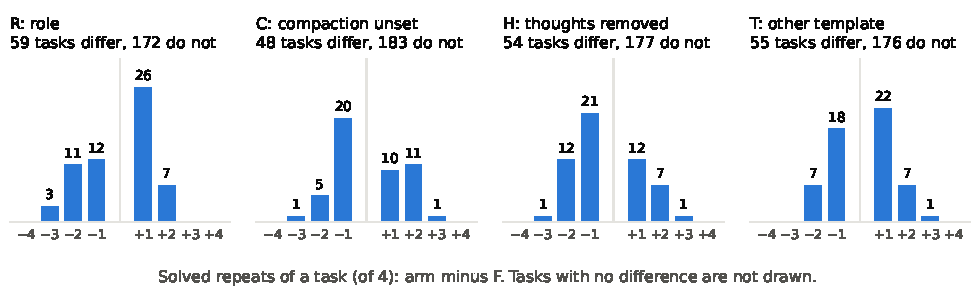
\includegraphics[width=\linewidth]{fig/supp_taskdiff.pdf}
\caption{Tasks whose number of solved repeats differs between an arm and F. Bars to the left of the centre line are
tasks with fewer solved repeats in the arm.}
\label{fig:s-taskdiff}
\end{figure}

\subsection{Secondary analysis: repositories}

Tasks of one repository tend to succeed and fail together, so the registered secondary analysis takes the \SRepos{}
repositories as its units (Table~\ref{tab:s-repolevel}). Table~\ref{tab:s-repos} and Figure~\ref{fig:s-repos} show
each repository. All four repository-level intervals include zero, and the smallest two-sided $p$ is \SMinRepoP{} (H).
The leave-one-repository-out estimates of H stay negative ($-\SHLooLo$ to $-\SHLooHi$ points), so no single
repository produces the estimate of H; those of R, C and T change sign.

\begin{table}[!htb]
\centering
\caption{Secondary analysis at the repository level (15 repositories): exact wild cluster bootstrap-$t$ with Rademacher weights, its inverted 95\% interval, the six-point (Webb) variant, a CR1 interval, the repository-equal estimate and the range of leave-one-repository-out estimates. Estimates in percentage points.}\label{tab:s-repolevel}
\footnotesize\setlength{\tabcolsep}{4pt}
\begin{tabular}{lrrrrrrr}
\toprule
Arm & \parbox[b]{1.9cm}{\raggedleft Repositories that differ} & Exact $p$ & Webb $p$ & 95\% interval & CR1 interval & \parbox[b]{1.9cm}{\raggedleft Repository-equal} & Leave-one-out range \\
\midrule
R & 12 & 0.8188 & 0.7780 & [${-}3.81$, ${+}2.38$] & [${-}2.70$, ${+}2.05$] & ${+}1.62$ & [${-}1.09$, ${+}0.36$] \\
C & 8 & 0.8438 & 0.7788 & [${-}0.88$, ${+}2.81$] & [${-}1.22$, ${+}1.65$] & ${+}4.02$ & [${-}0.22$, ${+}0.60$] \\
H & 12 & 0.1831 & 0.1736 & [${-}4.94$, ${+}1.56$] & [${-}4.65$, ${+}0.53$] & ${-}2.98$ & [${-}3.01$, ${-}1.44$] \\
T & 9 & 0.8047 & 0.7374 & [${-}1.44$, ${+}4.62$] & [${-}2.09$, ${+}3.61$] & ${+}2.65$ & [${-}0.55$, ${+}1.66$] \\
\bottomrule
\end{tabular}
\end{table}

\begin{table}[!htb]
\centering
\caption{The 15 repositories of the panel: tasks, runs solved in arm F (of four per task) and, per arm, the summed change against F in task-equivalents (solved runs divided by four).}\label{tab:s-repos}
\footnotesize
\begin{tabular}{lrrrrrr}
\toprule
Repository & Tasks & F solved runs & R & C & H & T \\
\midrule
\texttt{pypa/packaging} & 65 & 65 of 260 & ${+}0.50$ & ${-}0.50$ & ${-}2.00$ & ${-}1.00$ \\
\texttt{pydantic/pydantic-settings} & 48 & 27 of 192 & ${+}1.25$ & 0 & ${+}0.75$ & ${+}2.75$ \\
\texttt{python-poetry/tomlkit} & 35 & 31 of 140 & ${-}1.00$ & ${-}0.50$ & ${-}1.50$ & 0 \\
\texttt{more-itertools/more-itertools} & 23 & 39 of 92 & ${-}1.50$ & ${+}0.25$ & ${-}1.75$ & 0 \\
\texttt{pallets/click} & 22 & 13 of 88 & ${-}0.50$ & ${-}0.25$ & ${-}0.50$ & ${-}0.25$ \\
\texttt{pallets/werkzeug} & 9 & 3 of 36 & ${+}0.25$ & 0 & ${-}0.25$ & ${+}0.25$ \\
\texttt{mahmoud/boltons} & 7 & 12 of 28 & ${-}0.25$ & 0 & ${+}0.50$ & ${-}0.25$ \\
\texttt{jd/tenacity} & 6 & 9 of 24 & ${-}0.25$ & 0 & ${-}0.25$ & ${-}0.50$ \\
\texttt{pytest-dev/pluggy} & 6 & 3 of 24 & ${+}0.50$ & ${+}1.00$ & ${+}0.75$ & 0 \\
\texttt{python-humanize/humanize} & 3 & 11 of 12 & ${-}0.25$ & ${+}0.25$ & ${+}0.25$ & ${+}0.25$ \\
\texttt{hynek/structlog} & 2 & 2 of 8 & ${+}0.25$ & ${-}0.25$ & ${-}0.50$ & ${+}0.25$ \\
\texttt{python-attrs/attrs} & 2 & 0 of 8 & 0 & 0 & 0 & 0 \\
\texttt{jazzband/prettytable} & 1 & 1 of 4 & ${+}0.25$ & ${+}0.50$ & ${-}0.25$ & ${+}0.25$ \\
\texttt{marshmallow-code/marshmallow} & 1 & 0 of 4 & 0 & 0 & 0 & 0 \\
\texttt{python-attrs/cattrs} & 1 & 4 of 4 & 0 & 0 & 0 & 0 \\
\midrule
All & 231 & 220 of 924 & ${-}0.75$ & ${+}0.50$ & ${-}4.75$ & ${+}1.75$ \\
\bottomrule
\end{tabular}
\end{table}


\begin{figure}[!htb]
\centering
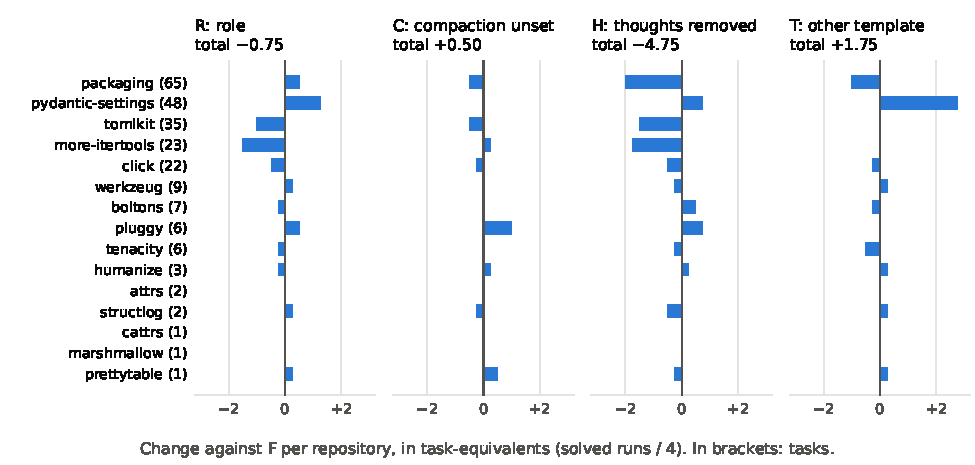
\includegraphics[width=\linewidth]{fig/supp_repos.pdf}
\caption{Change against F in each repository, per arm. Repositories are ordered by their number of tasks.}
\label{fig:s-repos}
\end{figure}

\subsection{Sensitivity analyses}

Three sensitivity analyses were registered with the primary one (Table~\ref{tab:s-sens}). The first treats the runs
that were unsolved at the five-minute limit as missing, in both arms; the estimate of H is then $\SHTimeCapMissing$
points ($p = \SHTimeCapMissingP$) instead of $-\SHd$. The other two score as unsolved every slot whose first job was
interrupted, in the arm or in F. No sensitivity analysis gives a $p$-value below 0.05.

\begin{table}[!htb]
\centering
\caption{Pre-registered sensitivity analyses of the primary estimate (percentage points; exact two-sided sign-flip $p$, unadjusted).}\label{tab:s-sens}
\footnotesize
\begin{tabular}{llrrrr}
\toprule
Arm & Analysis & Tasks & Runs affected & $d$ & Exact $p$ \\
\midrule
R & five-minute-limit runs of both arms treated as missing & 229 & 37 & ${-}0.29$ & 0.8652 \\
 & slots of the arm with an infrastructure row scored unsolved & 231 & 5 & ${-}0.43$ & 0.8011 \\
 & slots of F with an infrastructure row scored unsolved & 231 & 3 & ${-}0.22$ & 0.9321 \\
C & five-minute-limit runs of both arms treated as missing & 229 & 34 & ${+}0.22$ & 0.9253 \\
 & slots of the arm with an infrastructure row scored unsolved & 231 & 5 & ${+}0.11$ & 1.0000 \\
 & slots of F with an infrastructure row scored unsolved & 231 & 3 & ${+}0.32$ & 0.8506 \\
H & five-minute-limit runs of both arms treated as missing & 226 & 123 & ${-}1.25$ & 0.3414 \\
 & slots of the arm with an infrastructure row scored unsolved & 231 & 8 & ${-}2.16$ & 0.0980 \\
 & slots of F with an infrastructure row scored unsolved & 231 & 3 & ${-}1.95$ & 0.1270 \\
T & five-minute-limit runs of both arms treated as missing & 229 & 36 & ${+}0.76$ & 0.5604 \\
 & slots of the arm with an infrastructure row scored unsolved & 231 & 3 & ${+}0.76$ & 0.5604 \\
 & slots of F with an infrastructure row scored unsolved & 231 & 3 & ${+}0.87$ & 0.4947 \\
\bottomrule
\end{tabular}
\end{table}


\subsection{Exposure and the prompt check}

A divergence can only matter in the requests it changes. The frozen checker re-rendered all \SRequests{} returned
requests from the request dumps of the jobs. For each of the \SChecksPassed{} analysed runs it confirmed that the
prompts carry the divergence of the run's arm and no other difference; \SChecksFailed{} runs failed the check. The
divergence changed \SExposureMin{} to \SExposureMax\% of the requests in R, H and T, and \SCChanged\% in C
(Table~\ref{tab:s-exposure}).

\begin{table}[!htb]
\centering
\caption{Exposure: requests re-rendered by the frozen checker, and those whose rendered prompt the arm's divergence changed.}\label{tab:s-exposure}
\footnotesize
\begin{tabular}{lrrrrr}
\toprule
Arm & Runs & Requests checked & Changed by the divergence & Share (\%) & Failed calls recorded \\
\midrule
F & 924 & 15{,}043 & 0 & 0.0 & 17 \\
R & 924 & 15{,}290 & 13{,}616 & 89.1 & 20 \\
C & 924 & 13{,}036 & 2{,}709 & 20.8 & 131 \\
H & 924 & 17{,}450 & 15{,}684 & 89.9 & 112 \\
T & 924 & 14{,}787 & 12{,}629 & 85.4 & 19 \\
\bottomrule
\end{tabular}

\par\smallskip\parbox{0.96\linewidth}{\footnotesize No run has more than one failed call. Of the 299 failed calls, 178 are in runs unsolved at the five-minute limit, 115 in runs that ended on a rejected over-long prompt and 6 in solved runs.}
\end{table}


\subsection{Exploratory run measures}

Table~\ref{tab:s-measures} compares thirteen measures of a run between each arm and F. These comparisons were not
part of the registered tests and are not adjusted for multiplicity. H runs are longer: \SHTimeMean{}~s of agent time
on average against \SFTimeMean{}~s in F (medians \SHTimeMedian{} and \SFTimeMedian{}~s; Figure~\ref{fig:s-time}), with
\SHTokOut{} completion tokens per run against \SFTokOut.

\begin{table}[!htb]
\centering
\caption{Exploratory run measures: mean in arm F, and the paired difference of each arm against F; below it, its 95\% interval (CR1, repository clusters). No multiplicity adjustment.}\label{tab:s-measures}
\footnotesize\setlength{\tabcolsep}{3.5pt}
\begin{tabular}{lrrrrr}
\toprule
Measure & F mean & R $-$ F & C $-$ F & H $-$ F & T $-$ F \\
\midrule
history summaries per run & 0.69 & ${+}0.13$ & ${-}0.69$ & ${-}0.30$ & ${-}0.02$ \\
 &  & {\scriptsize [${+}0.04$, ${+}0.22$]} & {\scriptsize [${-}0.86$, ${-}0.53$]} & {\scriptsize [${-}0.47$, ${-}0.12$]} & {\scriptsize [${-}0.10$, ${+}0.06$]} \\[-2pt]
\addlinespace[2pt]% \\
runs with a summary (share) & 0.482 & ${+}0.038$ & ${-}0.482$ & ${-}0.161$ & ${-}0.014$ \\
 &  & {\scriptsize [${-}0.024$, ${+}0.099$]} & {\scriptsize [${-}0.572$, ${-}0.391$]} & {\scriptsize [${-}0.249$, ${-}0.073$]} & {\scriptsize [${-}0.059$, ${+}0.030$]} \\[-2pt]
\addlinespace[2pt]% \\
largest prompt (tokens) & 12{,}721 & ${+}220$ & ${+}2{,}160$ & ${-}1{,}499$ & ${-}95$ \\
 &  & {\scriptsize [${+}111$, ${+}329$]} & {\scriptsize [${+}1{,}666$, ${+}2{,}655$]} & {\scriptsize [${-}1{,}903$, ${-}1{,}095$]} & {\scriptsize [${-}284$, ${+}95$]} \\[-2pt]
\addlinespace[2pt]% \\
over-long prompt rejected (share) & 0.000 & ${+}0.000$ & ${+}0.123$ & ${+}0.001$ & ${+}0.000$ \\
 &  & {\scriptsize [${+}0.000$, ${+}0.000$]} & {\scriptsize [${+}0.075$, ${+}0.172$]} & {\scriptsize [${-}0.001$, ${+}0.003$]} & {\scriptsize [${+}0.000$, ${+}0.000$]} \\[-2pt]
\addlinespace[2pt]% \\
five-minute limit (share) & 0.018 & ${+}0.003$ & ${+}0.000$ & ${+}0.096$ & ${+}0.002$ \\
 &  & {\scriptsize [${-}0.005$, ${+}0.012$]} & {\scriptsize [${-}0.005$, ${+}0.005$]} & {\scriptsize [${+}0.073$, ${+}0.119$]} & {\scriptsize [${-}0.002$, ${+}0.006$]} \\[-2pt]
\addlinespace[2pt]% \\
tool-call budget reached (share) & 0.006 & ${+}0.003$ & ${-}0.005$ & ${+}0.013$ & ${-}0.002$ \\
 &  & {\scriptsize [${-}0.004$, ${+}0.011$]} & {\scriptsize [${-}0.012$, ${+}0.001$]} & {\scriptsize [${-}0.002$, ${+}0.028$]} & {\scriptsize [${-}0.006$, ${+}0.002$]} \\[-2pt]
\addlinespace[2pt]% \\
no submission (share) & 0.005 & ${-}0.004$ & ${-}0.003$ & ${-}0.004$ & ${+}0.001$ \\
 &  & {\scriptsize [${-}0.015$, ${+}0.006$]} & {\scriptsize [${-}0.013$, ${+}0.007$]} & {\scriptsize [${-}0.015$, ${+}0.006$]} & {\scriptsize [${-}0.010$, ${+}0.012$]} \\[-2pt]
\addlinespace[2pt]% \\
agent time (s) & 77.8 & ${+}3.9$ & ${-}11.2$ & ${+}58.9$ & ${-}1.2$ \\
 &  & {\scriptsize [${-}0.1$, ${+}7.9$]} & {\scriptsize [${-}14.7$, ${-}7.8$]} & {\scriptsize [${+}49.4$, ${+}68.3$]} & {\scriptsize [${-}6.5$, ${+}4.0$]} \\[-2pt]
\addlinespace[2pt]% \\
model calls & 16.28 & ${+}0.27$ & ${-}2.17$ & ${+}2.60$ & ${-}0.28$ \\
 &  & {\scriptsize [${-}0.25$, ${+}0.79$]} & {\scriptsize [${-}2.51$, ${-}1.83$]} & {\scriptsize [${+}1.31$, ${+}3.90$]} & {\scriptsize [${-}1.05$, ${+}0.50$]} \\[-2pt]
\addlinespace[2pt]% \\
failed model calls & 0.018 & ${+}0.003$ & ${+}0.123$ & ${+}0.103$ & ${+}0.002$ \\
 &  & {\scriptsize [${-}0.005$, ${+}0.012$]} & {\scriptsize [${+}0.077$, ${+}0.169$]} & {\scriptsize [${+}0.079$, ${+}0.127$]} & {\scriptsize [${-}0.002$, ${+}0.006$]} \\[-2pt]
\addlinespace[2pt]% \\
tool calls & 12.87 & ${+}0.19$ & ${-}1.23$ & ${+}2.52$ & ${-}0.23$ \\
 &  & {\scriptsize [${-}0.31$, ${+}0.70$]} & {\scriptsize [${-}1.42$, ${-}1.05$]} & {\scriptsize [${+}1.64$, ${+}3.41$]} & {\scriptsize [${-}0.92$, ${+}0.45$]} \\[-2pt]
\addlinespace[2pt]% \\
prompt tokens, summed & 136{,}123 & ${+}3{,}585$ & ${+}9{,}332$ & ${+}12{,}785$ & ${-}3{,}332$ \\
 &  & {\scriptsize [${-}1{,}493$, ${+}8{,}662$]} & {\scriptsize [${+}4{,}824$, ${+}13{,}841$]} & {\scriptsize [${+}443$, ${+}25{,}127$]} & {\scriptsize [${-}11{,}389$, ${+}4{,}725$]} \\[-2pt]
\addlinespace[2pt]% \\
completion tokens & 7{,}690 & ${+}440$ & ${-}1{,}253$ & ${+}6{,}707$ & ${-}245$ \\
 &  & {\scriptsize [${-}18$, ${+}899$]} & {\scriptsize [${-}1{,}635$, ${-}871$]} & {\scriptsize [${+}5{,}645$, ${+}7{,}768$]} & {\scriptsize [${-}796$, ${+}305$]} \\
\bottomrule
\end{tabular}
\end{table}


\begin{figure}[!htb]
\centering
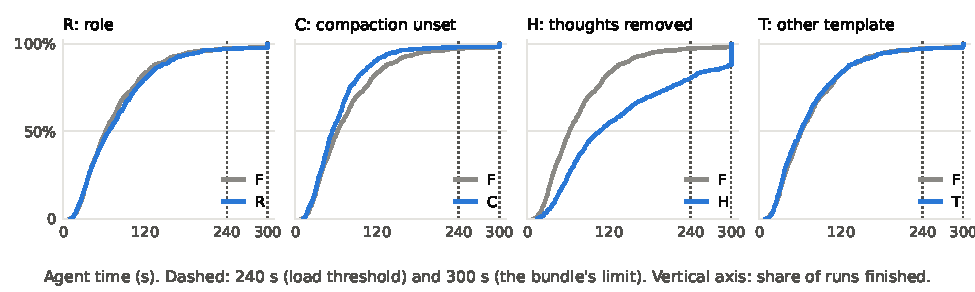
\includegraphics[width=\linewidth]{fig/supp_time.pdf}
\caption{Agent time per run: each arm (blue) against F (grey).}
\label{fig:s-time}
\end{figure}

\section{Applications of the pass rule}\label{sec:s-gates}

\begin{figure}[!tb]
\centering
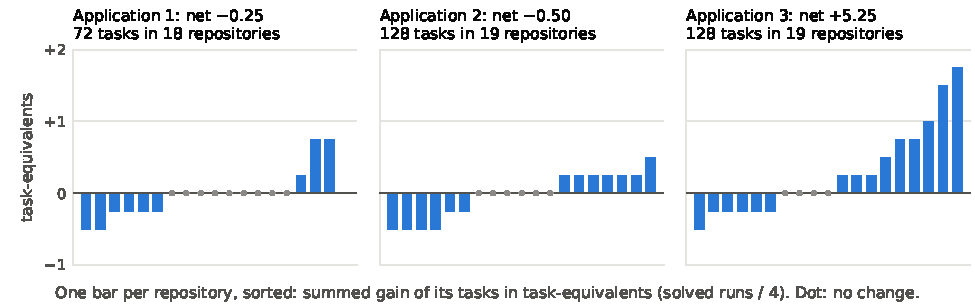
\includegraphics[width=\linewidth]{fig/supp_gates.pdf}
\caption{Gain of each repository in the three applications of the pass rule (candidate minus baseline). Repositories
are sorted by their total within each application.}
\label{fig:s-gates}
\end{figure}

\begin{table}[!htb]
\centering
\caption{Every application of the pass rule of Section 5 to a real candidate, from the frozen gate reports. Baseline and candidate are two versions of the withheld agent bundle.}\label{tab:s-gates}
\footnotesize
\begin{tabular}{lrrr}
\toprule
 & Application 1 & Application 2 & Application 3 \\
\midrule
Task set & small panel & large panel minus small & as application 2 \\
Tasks; repositories; repeats & 72; 18; 4 & 128; 19; 4 & 128; 19; 4 \\
Runs per arm (all with a result row) & 288 & 512 & 512 \\
Solved runs: baseline, candidate & 63, 62 & 103, 101 & 97, 118 \\
Mean gain (points; exact fraction) & ${-}0.35$ (${-}1/288$) & ${-}0.39$ (${-}1/256$) & ${+}4.10$ ($21/512$) \\
\quad (1) gain at least $2/58$ & not met & not met & met \\
Bootstrap-$t$; one-sided $p$ (9{,}999 draws) & ${-}0.175$; 0.6034 & ${-}0.366$; 0.6034 & ${+}1.954$; 0.0405 \\
One-sided $p$ by exact enumeration & 0.6113 & 0.6067 & 0.0360 \\
\quad (2) $p \le 0.025$ & not met & not met & not met \\
Repositories gaining; losing & 3; 6 & 7; 6 & 9; 6 \\
\quad (3a) at least three repositories gain & met & met & met \\
Lowest leave-one-repository-out gain (points) & ${-}1.47$ & ${-}0.85$ & ${+}2.94$ \\
\quad (3b) every leave-one-out gain positive & not met & not met & met \\
Agent time, candidate / baseline (s) & 68.4 / 66.6 & 89.3 / 75.6 & 79.4 / 72.0 \\
\quad (4a) ratio at most 1.2 & 1.026: met & 1.182: met & 1.103: met \\
Infrastructure rows: baseline, candidate & 0, 0 & 0, 0 & 0, 0 \\
\quad (4b) infrastructure errors do not rise & met & met & met \\
Worst repository total (task-equivalents) & ${-}0.50$ & ${-}0.50$ & ${-}0.50$ \\
\quad (5) no repository loses two or more & met & not registered & not registered \\
\midrule
Decision of the frozen rule & \textbf{FAIL} & \textbf{FAIL} & \textbf{FAIL} \\
\bottomrule
\end{tabular}
\end{table}


% Section "Applications of the pass rule": prose. Numbers: gen/gate_macros.tex (from the frozen gate reports). The
% screen counts (576, 288, five, two, 48; 25, 22 and 25 of 96 against 19, 21 and 20) come from the recorded screen
% analyses, and the statements on the history of the third candidate (two reads of earlier runs, six runs,
% one submission, score not arrived at the gate run) from its registration and its log. build_supp.py stops if a
% statement below on decisions, conditions, signs or task sets no longer holds.
The pass rule of \papersec{5} was applied \SGateCount{} to a real candidate: a changed version of the withheld
agent bundle, tested against the unchanged baseline on the same tasks and repeats. Each application ran once. Its rule,
tasks and analysis script were frozen before its first job, and the outcomes stayed unread until the run had ended.
Table~\ref{tab:s-gates} gives every quantity that the rule uses, and Figure~\ref{fig:s-gates} the gain of every
repository.

\paragraph{How the candidates were chosen.}
Each candidate was the leader of a screen on one separate 48-task set, with two repeats per task: 576 runs over the
baseline and five variants for the first candidate, and 288 runs over the baseline and two variants for each of the
other two. Each leader solved more runs than the baseline in its screen (25, 22 and 25 of 96, against 19, 21 and 20).
A screen selects a candidate and tests nothing, because the leader of several variants is expected to look better in
its screen than it is. No task of the screens is among the tasks of an application. Two small pilots came before the
screens of the later candidates. The variants of the second candidate were first tried on 15 tasks of the case-study
panel, which shares no task with an application. Two predecessors of the third candidate were tried on 16 tasks of the
small panel, that is, on tasks of the first application and on none of the second and third.

\paragraph{Tasks and conditions.}
The first application used the small panel (\SGateOneTasks{} tasks) and all five conditions of \papersec{5}. The
second used the \SGateTwoTasks{} tasks of the large panel that are outside the small one. The third used the same
\SGateThreeTasks{} tasks as the second, and both arms ran again. Its registration stated three things before the run:
that this was the second use of that task set, that the candidate had run on none of these tasks, and that the
candidate was built after the result of the second application was known. It also named two mechanical reads of
earlier runs that went into a repair of the candidate and that may include runs on these tasks: a scan of the
agent's commands in the \SGateTwoSessions{} runs of the second application, and the output of one command in six
earlier runs. Neither read used whether a task was solved. The candidate had been submitted to the competition
once before the run; its hosted score had not arrived when the outcomes were opened, and it is not an input of the
rule. The second and third applications registered conditions (1) to (4) only.

\paragraph{Results.}
The rule asks for a mean gain of at least \SGateMinGain{} points with a one-sided $p$ of at most \SGateAlpha, and for
further conditions on repositories, time and infrastructure errors. No candidate passed. The first two estimates are
below zero: \SGateOneGain{} points (\SGateOneCand{} against \SGateOneBase{} solved runs of \SGateOneRuns; $p =
\SGateOneP$) and \SGateTwoGain{} points (\SGateTwoCand{} against \SGateTwoBase{} of \SGateTwoRuns; $p = \SGateTwoP$).
The third candidate solved \SGateThreeMore{} runs more than the baseline (\SGateThreeCand{} against \SGateThreeBase{}
of \SGateThreeRuns), a gain of \SGateThreeGain{} points. This gain is above the required size, and conditions (3) and
(4) are met: \SGateThreeReposUp{} of the \SGateThreeRepos{} repositories gain, \SGateThreeReposDown{} lose, and the
lowest leave-one-repository-out gain is \SGateThreeLoo{} points. But the one-sided $p$ is \SGateThreeP, above
\SGateAlpha, so condition (2) is not met and the decision is FAIL.

\paragraph{How to read the decisions.}
The verdict of a failed application is ``not confirmed''. It is not evidence that the candidate has no effect: the
registration of the third application estimated, before the run, that a run of this size detects a true gain of the
required size about half of the time. Nor do we call the third candidate an improvement. Its $p$ is not corrected for
the three applications, and it is also above \SGateAlphaSplit, the level divided by three. Its gain is uneven: the
three repositories with the largest totals hold \SGateThreeTopThreeTasks{} of the \SGateThreeTasks{} tasks and gain
\SGateThreeTopThree{} task-equivalents, while the net gain over all repositories is \SGateThreeNet{}
(Figure~\ref{fig:s-gates}). A gain concentrated in a few repositories is the case in which the rule has little
power (\papertab{3}), and it is also what a few repositories can produce by chance. The first two leaders did not keep
their screen lead on new tasks; this is consistent with the selection effect that the rule exists to catch.


\section{Recomputing the case study with the released kit}\label{sec:s-repro}

The released table \texttt{e8\_compare\_table.csv} is in the input format of the \texttt{compare} module of the kit.
From a clone of the repository, two commands recompute the analysis:

\begin{verbatim}
pip install "./drydock-eval[compare]"
drydock-eval compare signflip e8_compare_table.csv --reference F --repeats 4
\end{verbatim}

We ran this command from the released source tree with the script \texttt{supp/reproduce.py}, which stops on any
mismatch. For all four arms the command returned the registered estimate, the exact $p$ as the same fraction, the
Holm-adjusted $p$ and every repository-level quantity of Table~\ref{tab:s-repolevel}.

Two quantities depend on Monte Carlo draws: the inverted intervals, and the Monte Carlo $p$ that is reported next to
the exact one. The draws are frozen (seed \SReproSeed), but which draw meets which task depends on the order of the
tasks. The registered analysis used the order of the panel file; the command sorts the task identifiers. With the
tasks in panel order, the routine of the kit returns the registered values to the last digit
(Table~\ref{tab:s-repro}). With the order of the command, the ends of the 95\% intervals move by at most
\SReproMoveNinetyFive{} points and those of the simultaneous intervals by at most \SReproMoveSim{} points. The largest
move is the upper end of the interval of H, $+\SReproHCmdHi$ instead of $+\SReproHRegHi$ points. The $p$-value of the
test is a step function of the shift, and across that stretch it stays between \SReproStepLo{} and \SReproStepHi{},
next to the 0.05 it is compared with. Both intervals include zero. The paper reports the registered intervals.

\begin{table}[!htb]
\centering
\caption{Reproduction with the released kit: the two quantities that depend on Monte Carlo draws. 95\% intervals of the change against F in percentage points, and the Monte Carlo $p$ that accompanies the exact $p$.}\label{tab:s-repro}
\footnotesize
\begin{tabular}{lrrrrrr}
\toprule
 & \multicolumn{3}{c}{95\% interval} & \multicolumn{3}{c}{Monte Carlo $p$} \\
\cmidrule(lr){2-4}\cmidrule(lr){5-7}
Arm & Registered & Kit, panel order & Kit command & Registered & Kit, panel order & Kit command \\
\midrule
R & [${-}2.82$, ${+}2.17$] & [${-}2.82$, ${+}2.17$] & [${-}2.80$, ${+}2.16$] & 0.8650 & 0.8650 & 0.8642 \\
C & [${-}2.03$, ${+}2.48$] & [${-}2.03$, ${+}2.48$] & [${-}2.04$, ${+}2.48$] & 0.9243 & 0.9243 & 0.9268 \\
H & [${-}4.45$, ${+}0.38$] & [${-}4.45$, ${+}0.38$] & [${-}4.45$, ${+}0.25$] & 0.1106 & 0.1106 & 0.1095 \\
T & [${-}1.42$, ${+}2.94$] & [${-}1.42$, ${+}2.94$] & [${-}1.42$, ${+}2.94$] & 0.5599 & 0.5599 & 0.5624 \\
\bottomrule
\end{tabular}
\end{table}


\section{Released data and code}\label{sec:s-data}

Table~\ref{tab:s-files} lists the data files and Table~\ref{tab:s-columns} the columns of the run file.

\paragraph{What the files hold.}
Outcome rows and analysis results only. They hold no prompt, request, patch, test output, error text or machine
detail: the script copies a fixed list of fields by name and nothing else.

\paragraph{What is withheld.}
The agent bundle, its prompts and the request dumps of the jobs stay private for now; their release is planned for
2026-12-03 (\papersec{9}). For that reason the two arms of each pass-rule application are named baseline and candidate.

\paragraph{Where.}
The kit is at \url{\repourl} (tag \texttt{v0.4.0}, Apache-2.0). The branch \texttt{paper} of the same repository holds
the sources of the paper and of this supplement, the scripts that write its tables and figures, and the data files
with their checksums.

\begin{table}[!htb]
\centering
\caption{Data files released with the paper.}\label{tab:s-files}
\footnotesize
\begin{tabular}{lrp{9.2cm}}
\toprule
File & Records & Content \\
\midrule
\texttt{e8\_runs.csv} & 4{,}636 & one line per result row of the case study: arm, task, repository, repeat, outcome, times, calls, tokens, prompt check \\
\texttt{e8\_compare\_table.csv} & 4{,}636 & the same rows in the input format of \texttt{drydock-eval compare} (seven columns) \\
\texttt{e8\_tasks.csv} & 231 & per task: repository and solved repeats (0 to 4) in each arm \\
\texttt{e8\_repositories.csv} & 15 & per repository: tasks, solved runs per arm, summed change against F \\
\texttt{e8\_summary.json} & -- & the analysis results behind Tables~\ref{tab:s-rates} to~\ref{tab:s-measures}, copied field by field from the frozen report \\
\texttt{pass\_rule\_applications.json} & 3 & the applications of the pass rule (Table~\ref{tab:s-gates}) \\
\bottomrule
\end{tabular}
\end{table}

\begin{table}[!htb]
\centering
\caption{Columns of \texttt{e8\_runs.csv}. The rows of interrupted jobs hold the first ten columns and the two times of day only.}\label{tab:s-columns}
\footnotesize
\begin{tabular}{lp{11.4cm}}
\toprule
Column & Content \\
\midrule
\texttt{batch} & 1 to 5: the batch of the block in which the job ran; batch 5 holds the re-runs \\
\texttt{stage} & 1, 2 or 3: the nested stage of the job list that holds the task (118, 37 and 76 tasks) \\
\texttt{arm} & F, R, C, H or T \\
\texttt{task} & task identifier in the public task collection the panel was drawn from \\
\texttt{repository} & repository of the task (owner/name); the unit of clustering \\
\texttt{repeat} & 1 to 4 \\
\texttt{attempt} & 1; 2 for the re-run of an interrupted job \\
\texttt{row\_class} & agent: an analysed run. infrastructure: an interrupted job, not analysed \\
\texttt{outcome\_id} & A00 solved; A01 unsolved, run completed; A02 tool-call budget reached; A05 unsolved at the five-minute limit; A06 no submission; A18 unsolved, over-long prompt rejected; I09 interrupted job \\
\texttt{resolved} & 1 if the run is solved (the tests of the task pass on the edits the run left), else 0 \\
\texttt{t\_agent\_s} & seconds of the agent phase of the job \\
\texttt{t\_setup\_s} & seconds of the setup phase, before the agent starts \\
\texttt{t\_verify\_s} & seconds of the grading phase; empty if no test was run \\
\texttt{model\_calls} & chat requests of the run that returned a response \\
\texttt{model\_calls\_failed} & chat requests of the run that raised an error instead \\
\texttt{tool\_calls} & tool calls made by the agent \\
\texttt{tokens\_in} & prompt tokens, summed over the requests of the run \\
\texttt{tokens\_out} & completion tokens, summed over the requests of the run \\
\texttt{max\_prompt\_tokens} & largest prompt of the run, in tokens \\
\texttt{summaries} & history summaries (compactions) made during the run \\
\texttt{patch\_chars} & characters of the diff the run left; 0 if none \\
\texttt{test\_exit} & exit status of the test command; 0 = tests passed; $-1$ = no test was run \\
\texttt{start\_utc} & start of the job (UTC) \\
\texttt{end\_utc} & end of the job (UTC) \\
\texttt{requests\_checked} & returned requests of the run that the frozen checker re-rendered \\
\texttt{requests\_changed} & of them, requests whose prompt the reference rule of arm F would render differently (the exposure count; 0 in F) \\
\texttt{check\_passed} & 1 if the run passed the prompt check \\
\bottomrule
\end{tabular}
\end{table}


\end{document}
